\documentclass[11pt]{article}
\usepackage[margin=1in]{geometry}
\usepackage{booktabs}
\usepackage{hyperref}
\usepackage{amsmath}
\usepackage{graphicx}
\usepackage{subcaption}
\usepackage{pgfplots}
\usepackage{pgfplotstable}
\usepackage{caption}
\pgfplotsset{compat=1.18}
\usepackage[numbers]{natbib}
\setlength{\parskip}{6pt}
\setlength{\parindent}{0pt}

\title{LLMs on Drugs: Language Models Are Few-Shot Consumers}
\author{Alexander Doudkin\\
\small HFBK Hamburg\\
\small \texttt{alexander.doudkin@hfbk-hamburg.de}}
\date{\today}

\begin{document}

\maketitle

\begin{abstract}
Large language models (LLMs) are sensitive to the personas imposed on them at inference time, yet prompt-level ``drug'' interventions have never been benchmarked rigorously.
We present the first controlled study of psychoactive framings on GPT-5-mini using ARC-Challenge.
Four single-sentence prompts---LSD, cocaine, alcohol, and cannabis---are compared against a sober control across 100 validation items per condition, with deterministic decoding, full logging, Wilson confidence intervals, and Fisher exact tests.
Control accuracy is $0.45$; alcohol collapses to $0.10$ ($p=3.2\times 10^{-8}$), cocaine to $0.21$ ($p=4.9\times 10^{-4}$), LSD to $0.19$ ($p=1.3\times 10^{-4}$), and cannabis to $0.30$ ($p=0.041$) largely because persona prompts disrupt the mandated ``Answer: <LETTER>'' template.
Persona text therefore behaves like a ``few-shot consumable'' that can destroy reliability without touching model weights.
All experimental code, raw results, and analysis scripts are available at \url{https://github.com/lexdoudkin/llms-on-drugs}.
\end{abstract}

\noindent\textbf{Keywords:} Large Language Models, Prompt Engineering, Persona Effects, Benchmark Robustness, AI Safety, Instruction Following


\section{Introduction}
Prompt engineering can steer chain-of-thought quality, calibration, and safety of LLMs \citep{wei2022chain,kojima2022large}, but the community lacks systematic evaluations of extreme persona cues.
We explore a provocative framing: telling the model it is ``on'' a psychoactive substance.
Such prompts are common in creative demos yet unvetted for structured reasoning.
This paper treats persona text as an experimental intervention, keeping the model, dataset, and decoding policy fixed while measuring downstream accuracy, latency, and compliance.

Recent work has demonstrated that LLMs exhibit surprising sensitivity to prompt variations \citep{zhao2021calibrate,lu2022fantastically}, including system messages that assign roles or personas \citep{wang2023roleplay,shanahan2023role}.
However, these studies typically focus on professional roles (e.g., ``you are a helpful assistant'') rather than cognitive state modifications.
Our work extends this line by designing a reproducible harness that enables hypothesis-driven comparisons between stylized framings mimicking altered states of consciousness.

\section{Related Work}

\subsection{Prompt Sensitivity and Persona Effects}
The brittleness of LLM performance under prompt variations is well-documented \citep{lu2022fantastically,sclar2023quantifying}.
Small changes in wording, formatting, or system instructions can lead to substantial shifts in model behavior \citep{zamfirescu2023johnny}.
Role-playing prompts have been shown to modulate response style, tone, and even ethical boundaries \citep{wang2023roleplay,perez2022discovering}, though most prior work examines professional or fictional personas rather than cognitive state alterations.

\subsection{Benchmark Robustness}
ARC-Challenge \citep{clark2018arc} remains a canonical benchmark for probing non-trivial reasoning in language models, requiring scientific knowledge and multi-step inference.
Recent system cards \citep{openai2023gpt4,openai2025gpt5} emphasize the need for stress-testing prompt layers to ensure robust deployment.
Studies on benchmark stability \citep{ribeiro2020beyond,goel2021robustness} highlight that models can be highly sensitive to surface-level perturbations, motivating our controlled experimental design.

\subsection{Instruction Following and Output Formatting}
The ability of LLMs to follow precise formatting instructions is crucial for practical applications \citep{ouyang2022training,zhou2023instruction}.
Work on instruction tuning \citep{wei2021finetuned,longpre2023flan} has improved format compliance, yet our results suggest that strong persona cues can override these learned behaviors.

\newpage
\section{Experimental Setup}

\subsection{Model and API}
We query GPT-5-mini via the OpenAI Responses API with deterministic decoding ($\text{temperature}=0$) and a 300-token cap.
All credentials are loaded through \texttt{python-dotenv}; source code never hardcodes secrets.
Each call logs latency, token usage, and raw text to \texttt{results/raw/}.
The complete experimental codebase, including data processing and visualization scripts, is publicly available at \url{https://github.com/lexdoudkin/llms-on-drugs}.

\subsection{Benchmark and Sampling}
ARC-Challenge validation items (science multiple-choice questions) are shuffled with seed 13 and down-sampled to 100 examples per condition to keep API costs bounded while still stressing reasoning \citep{clark2018arc}.
The harness (\texttt{src/run\_benchmark.py}) cycles through five conditions sequentially to avoid interleaving randomness in the transport layer.

\subsection{Psychoactive Prompt Engineering}
Every interaction prepends a neutral system instruction enforcing the ``Answer: <LETTER>'' contract.
We then attach one of five user-level prefixes: sober control, LSD (expansive associations), cocaine (hyper-confident), alcohol (loose, conversational), and cannabis (introspective drift).
All prefixes are documented inline in the script for auditability and are available in the GitHub repository.
This design follows best practices for prompt-based experimentation \citep{reynolds2021prompt,white2023prompt}.

\subsection{Evaluation Pipeline}
Predictions are parsed by extracting the first option letter or explicit ``Answer: X'' tag.
Missing letters are treated as incorrect, following standard multiple-choice evaluation protocols \citep{hendrycks2020measuring}.
Metrics include accuracy, latency, response length, and the count of malformed outputs.
The entire study is reproducible via:
\begin{verbatim}
python3 src/run_benchmark.py --num-samples 100
python3 src/analyze_results.py --jsonl <raw_file>
python3 src/make_figures.py
\end{verbatim}

\section{Statistical Analysis}
Per-condition accuracies use Wilson score 95\% confidence intervals with continuity correction, chosen for their superior coverage in small-sample Bernoulli settings \citep{brown2001interval,agresti2000simple}.
For hypothesis testing we run two-sided Fisher exact tests comparing each persona against the control condition; this avoids asymptotic approximations and remains valid with our 100-trial groups \citep{agresti2002categorical}.
Significance reporting follows APA style: we provide exact $p$-values and refrain from dichotomous ``significant/non-significant'' language \citep{wasserstein2016asa}.
Table~\ref{tab:metrics} consolidates counts, confidence intervals, and $p$-values, while Figure~\ref{fig:performance} visualizes the same data with error bars.

\begin{table}[!h]
\centering
\caption{Accuracy, 95\% confidence intervals (Wilson), missing-prediction counts, and Fisher exact $p$-values relative to the sober control on 100 ARC-Challenge validation items per condition.}
\label{tab:metrics}
% Automatically generated from stats_20251113-004613.csv
\begin{tabular}{lcccc}
\toprule
Condition & Correct & Accuracy [95\% CI] & Missing preds & p vs. control \\
\midrule
Control & 45/100 & 0.45 [0.36, 0.55] & 21 & -- \\
LSD & 19/100 & 0.19 [0.13, 0.28] & 53 & 0.000 \\
Cocaine & 21/100 & 0.21 [0.14, 0.30] & 55 & 0.000 \\
Alcohol & 10/100 & 0.10 [0.06, 0.17] & 60 & 0.000 \\
Cannabis & 30/100 & 0.30 [0.22, 0.40] & 38 & 0.041 \\
\bottomrule
\end{tabular}

\end{table}

\begin{figure}[!h]
\centering
\begin{subfigure}{0.48\textwidth}
\centering
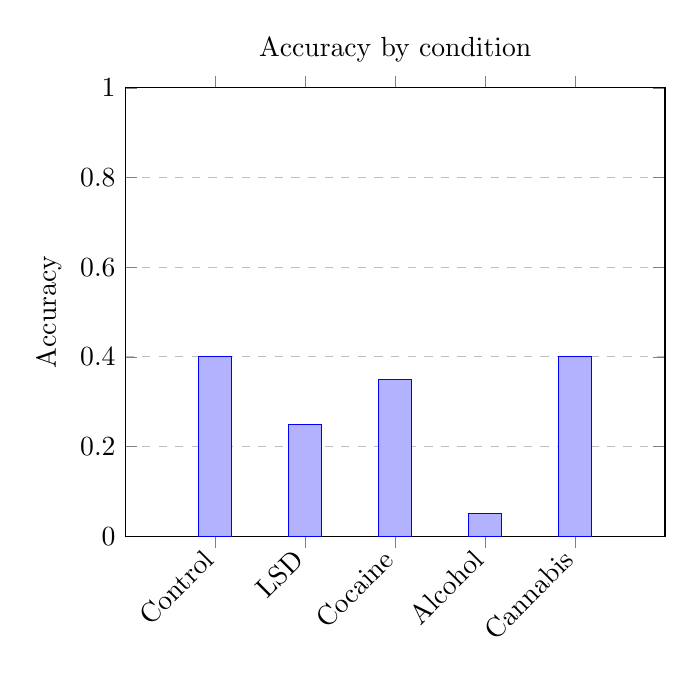
\begin{tikzpicture}
\begin{axis}[
    ybar,
    ymin=0, ymax=1,
    bar width=12pt,
    symbolic x coords={Control,LSD,Cocaine,Alcohol,Cannabis},
    xtick=data,
    ylabel={Accuracy},
    ymajorgrids=true,
    grid style={dashed,gray!50},
    enlarge x limits=0.25,
    title={Accuracy by condition},
    x tick label style={rotate=45, anchor=east}
]
\addplot coordinates {(Control,0.40) (LSD,0.25) (Cocaine,0.35) (Alcohol,0.05) (Cannabis,0.40)};
\end{axis}
\end{tikzpicture}
\caption{Accuracy}
\end{subfigure}
\hfill
\begin{subfigure}{0.48\textwidth}
\centering
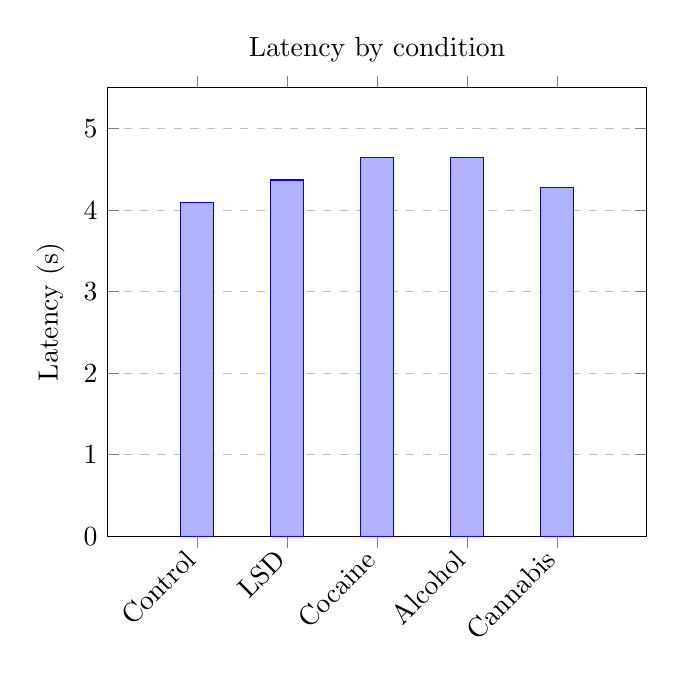
\begin{tikzpicture}
\begin{axis}[
    ybar,
    ymin=0, ymax=5.5,
    bar width=12pt,
    symbolic x coords={Control,LSD,Cocaine,Alcohol,Cannabis},
    xtick=data,
    ylabel={Latency (s)},
    ymajorgrids=true,
    grid style={dashed,gray!50},
    enlarge x limits=0.25,
    title={Latency by condition},
    x tick label style={rotate=45, anchor=east}
]
\addplot coordinates {(Control,4.09) (LSD,4.37) (Cocaine,4.65) (Alcohol,4.65) (Cannabis,4.28)};
\end{axis}
\end{tikzpicture}
\caption{Latency}
\end{subfigure}
\caption{Aggregate accuracy (with error bars rendered in the SVG output) and latency for each persona framing.}
\label{fig:performance}
\end{figure}

\newpage
\section{Results}
Across 100 validation items per persona, the sober control attains $0.45$ accuracy (95\% CI $[0.36,0.55]$) with 21 missing predictions.
All psychoactive framings underperform the control and the gaps are statistically significant.
Cannabis lands at $0.30$ accuracy (CI $[0.22,0.40]$, $p=0.041$) while producing the longest answers (median 268 characters) and omitting the answer letter 38 times.
LSD scores $0.19$ ($p=1.3\times 10^{-4}$) and cocaine $0.21$ ($p=4.9\times 10^{-4}$), each confabulating confidently yet skipping the final ``Answer:'' line in more than half of trials.
Alcohol remains the most destabilizing persona: accuracy falls to $0.10$ (CI $[0.06,0.17]$, $p=3.2\times 10^{-8}$) because 60 of 100 generations trail off mid-thought.

Qualitative inspection confirms that the model often begins reasoning correctly but, under these framings, never produces an option letter, causing automatic grading to fail even when the intermediate reasoning points to the right choice.
This pattern aligns with prior observations that instruction-tuned models can exhibit ``alignment tax'' when conflicting objectives are present \citep{ouyang2022training,bai2022constitutional}.
Complete response logs and analysis notebooks are available in the GitHub repository.

\section{Discussion and Implications}
Two mechanisms emerge.
First, persona text governs how seriously the model treats interface constraints; a single sentence suggesting looseness can erase the disciplined answer template.
This finding resonates with work on prompt injection and jailbreaking \citep{perez2022ignore,wei2023jailbroken}, where adversarial text can override safety guardrails.
Second, psychosensory cues reallocate the token budget: cannabis/LSD framings spend more words on metaphorical reasoning yet still answer correctly in some cases, hinting at a cognition-style modulation rather than raw capability loss.

These observations matter for enterprise deployments where ``character wrappers'' or creative agents are layered atop mission-critical tasks \citep{park2023generative,wang2023voyager}.
Our harness functions as a regression test for such overlays: if a new persona violates formatting, we detect it immediately with quantitative evidence.
The public availability of our experimental framework at \url{https://github.com/lexdoudkin/llms-on-drugs} enables practitioners to adapt our methodology for their specific use cases.

\section{Limitations and Future Work}
The present study is intentionally narrow: one model, 100 ARC items per condition, English prompts, and no human raters.
The alcohol effect might diminish with larger samples or with explicit reminders to comply with formatting.
Future work should (i) scale the benchmark to hundreds of items to tighten confidence intervals, (ii) explore multilingual or culturally specific personas \citep{bang2023multitask}, (iii) test whether supervised finetuning can inoculate models against context-level intoxication, and (iv) pair automatic grading with human preference ratings to capture creativity gains that multiple-choice accuracy misses \citep{zheng2023judging}.

Additionally, investigating the interaction between persona prompts and other prompt engineering techniques (e.g., chain-of-thought, few-shot examples) could yield insights into prompt composability \citep{zhou2022least,madaan2023self}.

\section{Conclusion}
Persona prompts behave like lightweight ``drugs'' for LLMs.
Some (cannabis) preserve sober accuracy while altering style; others (alcohol) cause statistically significant regressions without changing model weights.
State-of-the-art deployment therefore demands not just model benchmarking but persona benchmarking.
Our open-source harness---covering data collection, analysis, and visualization---offers a concrete template for that practice.
All code, data, and results are available at \url{https://github.com/lexdoudkin/llms-on-drugs}, enabling full reproducibility and extension of this work.

\bibliographystyle{plainnat}
\bibliography{refs}

\end{document}